%/////////////////////////////////////////////////
%/
\chapter{Incremental Linearization for Real Arithmetic}
%/
%/////////////////////////////////////////////////.
\label{chap:Incremental_Linearization_For_Real_Arithmetic}

%/////////////////////////////////////////////////
%/
\section{System Architecture}
%/
%/////////////////////////////////////////////////
\label{sec:system_architecture}
So far, we have seen the basic concepts to understand our thesis work and how the authors of \cite{Cimatti:2018:ILS:3274693.3230639} have performed incremental linearization (IL) for SMT Solver.
Figure \ref{fig:system_architecture_ours} depicts the whole process of our thesis work.\newline

\noindent The input is an NRA formula $\varphi$.
At first $\varphi$ is linearized to a LRA formula $\hat{\varphi}$ by a linearization method.
This linearization method follows the Algorithm \ref{alg:linearization} which we will explain later.
The formula $\hat{\varphi}$ is passed to the SMT solver and it results in either SAT with a satisfying solution $\hat{\mu}$ of $\hat{\varphi}$ or UNSAT or UNKNOWN.
SAT means the SMT solver finds $\hat{\varphi}$ is being satisfiable, UNSAT means $\hat{\varphi}$ is not satisfiable and UNKNOWN means the SMT solver is unable to determine the satisfiability  of $\hat{\varphi}$.
If the SMT solver results in either UNSAT or UNKNOWN, the method terminates.
Otherwise, it continues to work following the next step.\newline

\noindent The next step is to extend $\hat{\mu}$ to a model $\mu$ for assigning all variables in $\varphi$.
We have named $\mu$ as an estimated model.
If $\mu$ satisfies $\varphi$, it returns SAT and we are done.
Otherwise, we have to perform refinement over some predefined axioms to resist the spurious solutions of $\mu$.
This refinement process outputs a set $A$ of axioms that prevents the spurious solutions.
Finally, $\hat{\varphi}$ is augmented by conjuncting each axiom $\psi$ from the set $A$ and again $\hat{\varphi}$ is passed to the SMT solver.
This loop continues unless the SMT solver finds UNSAT or UNKNOWN for $\hat{\varphi}$ or the estimated model $\mu$ satisfies $\varphi$.\newline

% Define block styles
\tikzstyle{decision} = [diamond, draw, fill=yellow!20, 
    text width=4.5em, text badly centered, node distance=3cm, inner sep=0pt]
\tikzstyle{block} = [rectangle, draw, fill=blue!20, 
    text width=7em, text centered, rounded corners, minimum height=4em]
\tikzstyle{line} = [draw, -latex']
\tikzstyle{cloud} = [draw, ellipse,fill=red!20, node distance=3cm,
    minimum height=2em]
\begin{figure}
\centering
\begin{tikzpicture}[node distance = 2cm, auto]
    % Place nodes\node [block] ()
    \node [block] (nra) {NRA Formula, $\varphi$};
    \node [cloud, below=0.5cm of nra] (linearization) {Linearization};
    \node [block, below of=linearization] (lra) {LRA Formula, $\hat{\varphi}$};
    \node [cloud, below=0.5cm of lra] (smtsolver) {SMT Solver};
    \node [block, below of=smtsolver] (satmod) {SAT + Model ($\hat{\mu}$) of $\hat{\varphi}$};
    \node [block, right of=smtsolver, node distance=4cm] (unsatorunknown) {UNSAT / UNKNOWN};
    \node [block, below of=satmod] (ext) {Extend $\hat{\mu}$ to assign all variables in  $\varphi$};
    \node [cloud, left=1.5cm of ext] (formula) {$\hat{\varphi} := \hat{\varphi} \wedge \bigwedge\limits_{\psi \in A} \psi$};
    \node [decision, below=0.7 of ext] (decide) {$\mu \models \varphi ?$};
    \node [block, right of=decide, node distance=4cm] (sat) {SAT};
    \node [block, below=0.8cm of decide] (refinement) {Refinement for NRA};
    \node [cloud, below=0.5cm of refinement] (setofaxioms) {Set A of axioms unsatisfied under $\hat{\mu}$};
    % Draw edges
    \path [line] (nra) -- (linearization);
    \path [line] (linearization) -- (lra);
    \path [line] (lra) -- (smtsolver);
    \path [line] (smtsolver) -- (satmod);
    \path [line] (smtsolver) -- (unsatorunknown);
    \path [line] (formula) |- (smtsolver);
    \path [line] (satmod) -- (ext);
    \path [line] (ext) -- (decide);
    \path [line] (decide) -- node {No}(refinement);
    \path [line] (decide) -- node {Yes}(sat);
    \path [line] (refinement) -- (setofaxioms);
    \path [line] (setofaxioms) -| (formula);
\end{tikzpicture}
\caption{The incremental linearization process}
 \label{fig:system_architecture_ours}
\end{figure}

%/////////////////////////////////////////////////
%/
\section{Our Approach}
%/
%/////////////////////////////////////////////////
\label{sec:Our_Approach}
We have constructed an SMT-RAT module named \textit{NRAILModule} that linearizes an input NRA formula incrementally, solves it and utilizes the solution if the input NRA formula is not satisfied by it to make it satisfying via a refinement process.
SMT-RAT is an open source C++ toolbox for strategic and parallel SMT solving consisting of a collection of modules for solving quantifier-free (non)linear real and integer arithmetic formulas \cite{inproceedings}.\newline

\noindent Each of the modules of SMT-RAT implements a common interface.
The interface consists of some methods including addCore, checkCore. 
These methods are invoked by SMT-RAT in a defined manner.
The addCore($\varphi^\prime$) is invoked for each sub-formula $\varphi^\prime$ of the given input formula $\varphi$ by SMT-RAT at the beginning.
The checkCore() is invoked at the end to check the satisfiability of $\varphi$.
In our case, we perform linearization for each $\varphi^\prime$ in addCore($\varphi^\prime$) and the satisfiability checking logic with refinement process is formulated in checkCore().\newline

\begin{example}
\label{example:reorganization}
An example quantifier-free NRA formula:
$$\varphi := (3x^9y^2 -y < 5) \wedge (xy + 1 < 0)$$
SMT-RAT will reorganize this fomula as follows, we will use this example formula for other examples too:
$$\varphi := (3x^9y^2 + (-1)y + (-5) < 0) \wedge (xy + 1 < 0)$$
Here, the set of sub-formulas is, $\{3x^9y^2 + (-1)y + (-5) < 0, xy + 1 < 0\}$.
Each sub-formula from this set is denoted as $\varphi^\prime$.
\end{example}

\noindent To understand this paper, we do not need to know the internal methodology of SMT-RAT in depth.
We will explain SMT-RAT partly whenever we will need it to understand our work.
%/////////////////////////////////////////////////
%/
\subsection{addCore($\varphi^\prime$)}
%/
%/////////////////////////////////////////////////
\label{subsec:addCore}
The algorithm addCore($\varphi^\prime$) is shown in Algorithm \ref{alg:addcore}.
This addCore($\varphi^\prime$) is responsible for invoking the linearization method for each $\varphi^\prime$.
SMT-RAT has no module or method to linearize a formula.
That is why, we have introduced a method for linearization.
Also, SMT-RAT does not support UF.
So, in this work, one of our contributions is to adapt the linearization process by variables.\newline

\noindent Algorithm \ref{alg:addcore} is straightforward.
Whenever SMT-RAT runs \textit{NRAILModule}, at first, it calls addCore($\varphi^\prime$) for each $\varphi^\prime$.
Each $\varphi^\prime$ is linearized by linearization($\hat{\varphi}$) and linearized formula is collected into $\hat{\varphi}^\prime$ (line $1$).
Finally, addSubformulaToPassedFormula$( \hat{\varphi}^\prime )$ is invoked (line $2$) which adds $\hat{\varphi}^\prime$ to a global variable, $\hat{\varphi}$ of type list so that $\hat{\varphi}$ can be used for further computations from other methods, specially checkCore() as well.
So, we have got final linearized formula $\hat{\varphi}$ of $\varphi$.\newline

\begin{algorithm}
\caption{The algorithm addCore} 
\label{alg:addcore}
addCore($\varphi^\prime$)
\begin{algorithmic}[1]
\State $\hat{\varphi}^\prime :=$ linearization($\varphi^\prime$)
\State addSubformulaToPassedFormula $( \hat{\varphi}^\prime )$
\State \textbf{return} true
\end{algorithmic}
\end{algorithm}
%/////////////////////////////////////////////////
%/
\subsubsection{Linearization}
%/
%/////////////////////////////////////////////////
\label{subsubsec:Linearization}
\noindent The basic idea is to abstract each multiplication term (i.e., $x \ast x$, $x \ast y$ and so on) in a formula by a new variable called $z-variable$ (i.e., $z_1, z_2,\dots, z_i \hspace{1mm}\text{for some}\hspace{1mm} i \in \mathbb{N}$).
The abstraction is performed incrementally until the formula is linearized.
Algorithm for linearization is shown in Algorithm \ref{alg:linearization}.\newline

\noindent First, for each constraint $c$ from $\varphi^\prime$ (lines $1$ to $17$) and then collect left hand side of $c$ which is basically a polynomial $p$ (line $2$).
A variable $i$ and $j$ are initialized to $0$ which will be later used as the index of two different lists (line $3$ and $4$ respectively).\newline

\noindent Now, the algorithm enters a loop for each term $t \in p$ (lines $5$ to $14$).
At each iteration, it is checked whether $t$ is a constant or $t$ is linear or $t$ is non-linear.
If $t$ is a constant or linear (line $5$), then it is added as a linear term to a vector $\hat{p}$ (line $7$).
If the condition of the if block is false meaning that $t$ is non-linear, then the else block applies (lines $8$ to $12$).\newline

\begin{algorithm}
\caption{The algorithm linearization} 
\label{alg:linearization}
linearization($\varphi^\prime$)
\begin{algorithmic}[1]
\State for each constraint $c \in \varphi^\prime$
\State $\hspace{5mm}$ $p:=$ left hand side of $c$
\State $\hspace{5mm}$ $i:= 0$
\State $\hspace{5mm}$ $j:= 0$
\State $\hspace{5mm}$ \textbf{for each} term $t \in p$:
\State $\hspace{10mm}$ \textbf{if} $t$ is a constant $|| \hspace{1mm} t$ is linear:
\State $\hspace{15mm}$ $\hat{p}[i] := t$
\State $\hspace{10mm}$ \textbf{else}
\State $\hspace{15mm}$ $m:=$ monomial of $t$
\State $\hspace{15mm}$ $a:=$ coefficient of $t$
\State $\hspace{15mm}$ $z:=$ abstractMonomial($m$)
\State $\hspace{15mm}$ $\hat{p}[i] := a \ast z$
\State $\hspace{10mm} i\verb!++!$
\State $\hspace{5mm}$ end
\State $\hspace{5mm}$ $\hat{\varphi}^\prime[j] :=$ createFormula$( \hat{p},$ relational operator in $c)$
\State $\hspace{5mm}$ $j\verb!++!$
\State end
\State \textbf{return} $\hat{\varphi}^\prime$
\end{algorithmic}
\end{algorithm}

\noindent In line $9$ and $10$, we extract the monomial $m$ and the coefficient $a$ from $t:= a \ast m$, respectively.
After that, abstractMonomial($m$) is invoked which returns a variable $z$ that is used as an abstraction $m$ (line $11$).
abstractMonomial($m$) is explained briefly in Section \ref{subsubsec:Abstract_A_Monomial_IncrementallyBy_Z-variables}.
The variable $z$ is achieved by replacing each univariate multiplication term of $m$ recursively as follows:
$$\underbrace{ \underbrace{ \underbrace{ \underbrace{ x \ast x }\limits_{z_{1}} \ast \underbrace{ x \ast x }\limits_{z_{1}}}\limits_{z_{2}} \ast \underbrace{ \underbrace{ x \ast x }\limits_{z_{1}} \ast \underbrace{ x \ast x }\limits_{z_{1}}}\limits_{z_{2}}}\limits_{z_{3}} \ast x}\limits_{z \hspace{1mm} \to \hspace{1mm} z_{4}}$$
In multivariate monomials, first all univariate terms $x^d$ are abstracted, resulting in products $z_1, \dots z_i$, in which we iteratively abstract each multiplication by another fresh variable from left to right (see Equation \ref{eqn:abstractMonomial}, Example \ref{example:linearization}).
In line $12$ the linear abstraction $a \ast z$ is added to the list $\hat{p}$ at position $i$.
Finally, $i$ is incremented by 1 (line $13$) and the loop continues if there are other terms left in $p$.\newline

\noindent After termination of the inner loop, in line $15$ a linear constraint is created by building a sum of the terms in $\hat{p}$ and comparing it to $0$ according to the comparison operator of $c$.
This linear constraint is added to the list $\hat{\varphi}^\prime$ at position $j$.
Note that due to the reorganization of $\varphi$ by SMT-RAT shown in the Example \ref{example:reorganization}, the left-hand side of $c$ is always a sum of terms, the latter being products of a constant and variables.
Then $j$ is incremented by 1 (line $16$) and the outer loop continues if there are other constraints left in $\varphi^\prime$.
Lastly, in line $18$, the algorithm returns $\hat{\varphi}^\prime$.\newline

\begin{example}
\label{example:linearization}
Consider the same example formula as in the Example \ref{example:reorganization}:
$$\varphi := (3x^9y^2 + (-1)y + (-5) < 0) \wedge (xy + 1 < 0)$$
At first, linearization($\varphi^\prime$) is invoked for $\varphi^\prime := (3x^9y^2 + (-1)y + (-5) < 0)$ (line $1$, Algorithm \ref{alg:addcore}).\newline
Now,\newline 
constraint $c := (3x^9y^2 + (-1)y + (-5) < 0)$\newline
left hand side $p := 3x^9y^2 + (-1)y + (-5)$ (line $2$, Algorithm \ref{alg:linearization})\newline
terms are: $3x^9y^2, (-1)y$ and $-5$\newline

\noindent Now, for each term $t$ the for loop will be run (line $5$ to $14$, Algorithm \ref{alg:linearization}):
\begin{itemize}
	\item For $t := 3x^9y^2$ (line $9$ to $12$):
	$$\text{monomial }m := x^9y^2 \text{ and coefficient } a := 3$$
	This monomial is linearized as follows according to Algorithm \ref{alg:abstractMonomial}:
	\begin{align}
	    \underbrace{ \underbrace{ \underbrace{ \underbrace{ \underbrace{ x \ast x }\limits_{z_{1}} \ast \underbrace{ x \ast x }\limits_{z_{1}}}\limits_{z_{2}} \ast \underbrace{ \underbrace{ x \ast x }\limits_{z_{1}} \ast \underbrace{ x \ast x }\limits_{z_{1}}}\limits_{z_{2}}}\limits_{z_{3}} \ast x}\limits_{z_{4}} \ast \underbrace{ y \ast y }\limits_{z_{5}}}\limits_{z_{6}} \label{eqn:abstractMonomial}
	\end{align}
	$$\text{So, }z := z_{6}\text{ and } \hat{p}[0] := 3 \ast z_{6} \quad (i = 0)$$
    \item For $t := (-1)y$, $t$ is already linear (line $7$):
    $$\hat{p}[1] := (-1)y \quad (i = 1)$$
    \item For constant term $t := -5$ (line $7$):
    $$\hat{p}[2] := -5 \quad (i = 2)$$
So,
$$\text{linearized polynomial} \quad \hat{p} := z_{6} + (-1)y + (-5)$$
$$\text{linearized subformula} \quad \hat{\varphi}^\prime := ( z_{6} + (-1)y + (-5) < 0 )$$
Then $\hat{\varphi}^\prime$ is returned to addCore($\varphi^\prime$) and $\hat{\varphi}^\prime$ is inserted to $\hat{\varphi}$ by addSubformulaToPassedFormula $( \hat{\varphi}^\prime )$ (line $2$, Algorithm \ref{alg:addcore}).
In the same way, linearization($\varphi^\prime$) is again invoked for $\varphi^\prime:= x \ast y + 1$ (line $1$, Algorithm \ref{alg:addcore}) and  we get linear subformula $( z_{7} + 1 < 0 )$ as follows:
$$(\underbrace{ x \ast y }\limits_{z_{7}} + 1 < 0)$$
Finally, we get the linearized formula for $\varphi$:
$$\hat{\varphi} := ( z_{6} + (-1)y + (-5) < 0 ) \wedge ( z_{7} + 1 < 0 )$$
\end{itemize}
\end{example}
%/////////////////////////////////////////////////
%/
\subsubsection{Abstract a Monomial Incrementally by Z-variables}
%/
%/////////////////////////////////////////////////
\label{subsubsec:Abstract_A_Monomial_IncrementallyBy_Z-variables}
In the previous section, we have seen how the linearization process works and when abstractMonomial($m$) is called.
We have also seen how abstractMonomial($m$) method is executed and what this method returns (see Equation \ref{eqn:abstractMonomial}, Example \ref{example:linearization}). 
Encapsulating $m$ incrementally by Z-variables is the core of whole linearization proces.
In this section, we are going to see the algorithm behind this abstraction of $m$.\newline

\begin{algorithm}
\caption{The algorithm abstractMonomial} 
\label{alg:abstractMonomial}
abstractMonomial($m$)
\begin{algorithmic}[1]
\State $vList :=$ empty list
\State \textbf{for each} variable $v$ with $v^d \in m$ where $d$ is a positive integer:
\State \hspace{5mm} $vList$.pushBack(abstractUnivariateMonomial$(v, d)$)
\State end
\State $z :=$ abstractProductRecursively$(vList)$
\State \textbf{return} $z$
\end{algorithmic}
\end{algorithm}

\noindent The main idea of Algorithm \ref{alg:abstractMonomial} is to replace each univariate multiplication term (i.e., $x^2$ or $y^2$) $v^d$ in a monomial $m$ where $d \text{ is a positive integer}$ by $z-variable$, this $z-variable$ remains the same for each multiplication term ($x^2$) of $x$ where $x \in v$ means $x$ is the original variable.
We have mentioned the variable as original variable if it is contained in the input formula, $\varphi$.
This replacement continues until in the input monomial $m = x_{1}^{d_{1}}, \dots,x_{n}^{d_{n}}$ with $d_i \geq 1$ for all $i = 1, \dots, n$, we introduced an abstraction variable $z_i$ for each $x_i$ with $d_i > 1$.
Finally, the product of these abstraction variables and all $x_i$ with $d_i = 1$ is abstracted and returned to the caller method linearization($\varphi^\prime$) (see Equation \ref{eqn:vList}, Algorithm \ref{alg:abstractProductRecursively})\newline 

\begin{algorithm}
\caption{The algorithm abstractProductRecursively} 
\label{alg:abstractProductRecursively}
abstractProductRecursively$(vList)$
\begin{algorithmic}[1]
\While {($vList$.size() $> 1$)}
\State $first:= vList$.popFront() 
\State $second:= vList$.popFront()
\State $z:= first \ast second$
\State $vList$.pushFront($z$)
\EndWhile
\State \textbf{return} $vList$.front()
\end{algorithmic}
\end{algorithm}

\begin{align}
    \underbrace{ \underbrace{ \underbrace{ vList_{0} \hspace{5mm} \ast \hspace{5mm} vList_{1} }\limits_{z_{j}} \hspace{5mm} \ast \hspace{5mm} vList_{2} }\limits_{{z_{j+1}}_{\vdots}} \hspace{5mm} \ast \hspace{5mm} \dots \hspace{5mm} \ast \hspace{5mm} vList_{i}}\limits_{z \hspace{1mm} \to \hspace{1mm} z_{j+i-1}} \hspace{5mm} \label{eqn:vList}
\end{align}

\noindent Here, $i$ is a non-negative integer and $j$ is a positive integer.
%/////////////////////////////////////////////////
%/
\subsubsection{Abstraction of Univariate Monomial}
%/
%/////////////////////////////////////////////////
\label{subsubsec:abstractUnivariateMonomial}
\begin{sloppypar}
From the Section \ref{subsubsec:Abstract_A_Monomial_IncrementallyBy_Z-variables}, we have got to know that each $v^d$ in a monomial $m$ is abstracted by a fresh variable (line $3$, Algorithm \ref{alg:abstractMonomial}).
The using abstractUnivariateMonomial($v, d$) is in Algorithm \ref{alg:abstractUnivariateMonomial}.
The first if block runs when the input is already a single variable $v$ that does not need to be abstracted (lines $1$ to $2$).
In this case, the algorithm returns $m$ (lines $7$ to $8$).
In this algorithm, the most interesting part is the abstractUnivariateMonomialForEvenExponent$(v, d)$ (line $4$) and abstractUnivariateMonomialForOddExponent$(v, d)$ (line $6$).\newline
\end{sloppypar}

\begin{algorithm}
\caption{The algorithm abstractUnivariateMonomial} 
\label{alg:abstractUnivariateMonomial}
abstractUnivariateMonomial($v, d$)
\begin{algorithmic}[1]
\State \textbf{if} $d = 1$:
\State $\hspace{5mm}$ $m := v$
\State \textbf{else if} $d \hspace{1mm}\%\hspace{1mm} 2 == 0$:
\State $\hspace{5mm}$ $m :=$ abstractUnivariateMonomialForEvenExponent$(v, d)$
\State \textbf{else}
\State $\hspace{5mm}$ $m :=$ abstractUnivariateMonomialForOddExponent$(v, d)$
\State \textbf{if} $m$ is linear:
\State $\hspace{5mm}$  \textbf{return} $m$
\State let $v$ be the variable of $m$
\State let $d$ be the exponent of $m$
\State \textbf{return} abstractUnivariateMonomial$(v, d)$
\end{algorithmic}
\end{algorithm}

\noindent Lines $3$ to $4$ run if the remainder of $d \hspace{1mm}\%\hspace{1mm} 2$ is equal to $0$ means that $d$ is an even exponent.
As $d$ is an even exponent, there must be even numbers of $v$.
So, each pair of $v$ will be easily replaced by the same $z-variable$ (line $2$, Algorithm \ref{alg:abstractUnivariateMonomialForEvenExponent}) and a new monomial $m$ is being created (line $3$, Algorithm \ref{alg:abstractUnivariateMonomialForEvenExponent}):
\begin{align}
    m &:= z^{d^{\prime}} \hspace{5mm} ;\hspace{1mm}(d^\prime := \frac{d}{2}) \label{eqn:mPrime}
\end{align}
This $m$ is returned by abstractUnivariateMonomialForEvenExponent$(v, d)$ (line $4$, Algorithm \ref{alg:abstractUnivariateMonomialForEvenExponent}).
It is not necessary for $m$ to be always linear.
Sometimes. $m$ maybe linear.
If $m$ is linear, the algorithm returns $m$ (line $7$ to $8$).
Otherwise, $m$ has the form $z^{d^{\prime}}$ (lines $9$ and $10$).
\begin{align}
    v &:= z-variable \hspace{5mm} ;\hspace{1mm}(z-variable \in \hat{m}) \label{eqn:v} \\
    d &:= d^\prime \label{eqn:d}
\end{align}
Then Algorithm \ref{alg:abstractUnivariateMonomial} makes a recursive call to itself with parameters $z$ and $d^\prime$ (line $11$).\newline

\begin{example}
\label{example:even}
Let us consider a variable $x$ with an even exponent $d = 8$.
So, abstractUnivariateMonomialForEvenExponent$(x, 8)$ executes as follows:
	$$\underbrace{ x \ast x }\limits_{z_{1}} \ast \underbrace{ x \ast x }\limits_{z_{1}} \ast \underbrace{ x \ast x }\limits_{z_{1}} \ast \underbrace{ x \ast x }\limits_{z_{1}}$$
	$$m := z_{1}^4 \hspace{5mm} ;\hspace{1mm}(d^\prime := \frac{8}{2} = 4)$$
	Here, $m$ is not linear. 
	That is why a recursive call is made by the caller method with parameters $z_{1} \text{ and } 4$ (line $11$).
\end{example}

\begin{algorithm}
\caption{The algorithm abstractUnivariateMonomialForEvenExponent} 
\label{alg:abstractUnivariateMonomialForEvenExponent}
abstractUnivariateMonomialForEvenExponent($v, d$)
\begin{algorithmic}[1]
\State $d^\prime := d/2$
\State $z:= v^2$
\State $m := z^{d^\prime}$
\State \textbf{return} $m$
\end{algorithmic}
\end{algorithm}

\begin{sloppypar}
\noindent Now, line $5$ to $6$ runs if the remainder of $d \hspace{1mm}\%\hspace{1mm} 2$ is equal to $1$ means that $d$ is an odd exponent.
For this, the execution process of abstractUnivariateMonomialForOddExponent$(v, d)$ (Algorithm \ref{alg:abstractUnivariateMonomialForOddExponent}) is different than abstractUnivariateMonomialForEvenExponent$(v, d)$ (Algorithm \ref{alg:abstractUnivariateMonomialForEvenExponent}).
As $d$ is an odd exponent, one $v$ must be left after replacing each pair of $v$ by the same $z-variable$.
This $v$ which does not take part in the replacement is pushed into the front of a list $extraVList$.
A new monomial $m$ is created here too as in equation \ref{eqn:mPrime}.
For $m$, a while loop runs until it does not become linear by invoking either abstractUnivariateMonomialForEvenExponent$(z, d^\prime)$ or abstractUnivariateMonomialForOddExponent$(z, d^\prime)$.
Once, we get $m$ as linear, the variable of $m$ is pushed in the front of the $extraVList$.
Then the same replacement procedure as equation \ref{eqn:vList} occurs for $extraVList$ too from left to right and we get a single $z-variable$.
A linear monomial $m := z$ is created and finally, abstractUnivariateMonomialForOddExponent$(v, d)$ returns it (line $16$, algprithm \ref{alg:abstractUnivariateMonomialForOddExponent}) to the caller method.
The caller method is whether  abstractUnivariateMonomial($v, d$) (line $6$, Algorithm \ref{alg:abstractUnivariateMonomial}) or abstractUnivariateMonomialForOddExponent$(v, d)$ (line $11$, algprithm \ref{alg:abstractUnivariateMonomialForOddExponent}).\newline
\end{sloppypar}

\begin{algorithm}
\caption{The algorithm abstractUnivariateMonomialForOddExponent} 
\label{alg:abstractUnivariateMonomialForOddExponent}
abstractUnivariateMonomialForOddExponent($v, d$)
\begin{algorithmic}[1]
\State $extraVList :=$ empty list
\State $d^\prime := d/2$
\State $z:= v^2$
\State $extraVList$.pushFront($v$)
\State $m := z^{d^\prime}$
\While {($m$ is not linear)}
\State let $v$ be the variable of $m$
\State let $d$ be the exponent of $m$
\State \textbf{if} $d \hspace{1mm}\%\hspace{1mm} 2 == 0$::
\State $\hspace{5mm}$ $m :=$ abstractUnivariateMonomialForEvenExponent$(v, d)$
\State \textbf{else}
\State $\hspace{5mm}$ $m :=$ abstractUnivariateMonomialForOddExponent$(v, d)$
\EndWhile
\State \textbf{if} $m$ is linear:
\State  $\hspace{5mm}$ $extraVList$.pushFront(variable of $m$)
\State $\hspace{5mm}$  $z :=$ abstractProductRecursively$(extraVList)$
\State $\hspace{5mm}$ $m := z$
\State \textbf{return} $m$
\end{algorithmic}
\end{algorithm}

\begin{example}
\label{example:odd}
Let us consider a variable $x$ with an odd exponent, $d = 7$.
So, abstractUnivariateMonomialForOddExponent$(x, 7)$ executes as follows:

\tikzset{every picture/.style=remember picture}
\begin{figure}[H]
\centering
\begin{tikzpicture}[square/.style={regular polygon,regular polygon sides=4}]
    \node [] (equation) {$\underbrace{ x \ast x }\limits_{z_{1}} \ast \underbrace{ x \ast x }\limits_{z_{1}} \ast \underbrace{ x \ast x }\limits_{z_{1}} \ast \hspace{1mm}x$};
    \node [square,inner sep=0.4cm,draw, right=1cm of equation] (sq) {};
    \node[above = 0.3cm of sq] (lable) {extraVList};
    \path [>=stealth, ->]
     (equation) edge [bend left=10] (sq);
\end{tikzpicture}
\end{figure}
    
    $$m := z_{1}^3 \hspace{5mm} ;\hspace{1mm}(d^\prime := \frac{7}{2} = 3)$$
    Now, the while loop starts:
    \begin{itemize}
        \item Loop $1$: $m$ has odd exponent and abstractUnivariateMonomialForOddExponent$(z_{1}, 3)$ is called:
        
\tikzset{every picture/.style=remember picture}
\begin{figure}[H]
\centering
\begin{tikzpicture}[square/.style={regular polygon,regular polygon sides=4}]
    \node [] (equation) {$\underbrace{ z_{1} \ast z_{1} }\limits_{z_{2}} \ast \hspace{1mm}z_{1}$};
    \node [square,inner sep=0.4cm,draw, right=1cm of equation] (sq) {$x$};
    \node[above = 0.3cm of sq] (lable) {extraVList};
    \path [>=stealth, ->]
     (equation) edge [bend left=16] (sq);
\end{tikzpicture}
\end{figure}
        
        $$m := z_{2} \hspace{5mm} ;\hspace{1mm}(d^\prime := \frac{3}{2} = 1)$$
    \end{itemize}
    As $m$ is linear, $z_{2}$ is pushed into the front of $extraVList$ and the loop terminates.
    To get the single and final $z-variable$, the product of each two elements of $extraVList$ are replaced as follows:
    
\tikzset{every picture/.style=remember picture}
\begin{figure}[H]
\centering
\begin{tikzpicture}[square/.style={regular polygon,regular polygon sides=4}]
    \node [] (equation) {$\underbrace{ \underbrace{ z_{2} \ast z_1}\limits_{z_{3}} \ast \hspace{1mm}x}\limits_{z_{4}}$};
    \node [square,inner sep=0.4cm,draw, right=1cm of equation] (sq1) {$z_{2}$};
    \node [square,inner sep=0.4cm,draw, right=0.1mm of sq1] (sq2) {$z_{1}$};
    \node [square,inner sep=0.45cm,draw, right=0.1mm of sq2] (sq3) {$x$};
    \node[above = 0.3cm of sq2] (lable) {extraVList};
\end{tikzpicture}
\end{figure}
    
    $$m := z_{4}$$
\end{example}

\begin{sloppypar}
\noindent Notice that abstractUnivariateMonomialForEvenExponent$(v, d)$ may not return a linear monomial (example \ref{example:even}), whereas abstractUnivariateMonomialForOddExponent$(v, d)$ always returns a linear monomial (example \ref{example:odd}).\newline
\end{sloppypar}

\begin{example}
\label{example:abstractUnivariateMonomial}
    In the example \ref{example:linearization}, we have seen how a monomial $x^9y^2$ is linearized in an abstract way (equation \ref{eqn:abstractMonomial}).
    In this example, we will see how the Algorithms \ref{alg:abstractMonomial} and \ref{alg:abstractUnivariateMonomial} are executed to linearize the monomial $x^9y^2$.
    When abstractMonomial($x^9y^2$) is invoked it executes as follows: 
    \begin{itemize}
        \item For $x^9$ in $m$ abstractUnivariateMonomial($x, 9$) is invoked (line $3$, Algorithm \ref{alg:abstractMonomial}).
        The exponent $9$ is odd.
        So, abstractUnivariateMonomialForOddExponent$(x, 9)$ is executed (line $6$, Algorithm \ref{alg:abstractUnivariateMonomial}):
        
\tikzset{every picture/.style=remember picture}
\begin{figure}[H]
\centering
\begin{tikzpicture}[square/.style={regular polygon,regular polygon sides=4}]
    \node [] (equation) {$\underbrace{ x \ast x }\limits_{z_{1}} \ast \underbrace{ x \ast x }\limits_{z_{1}} \ast \underbrace{ x \ast x }\limits_{z_{1}}  \ast \underbrace{ x \ast x }\limits_{z_{1}} \ast \hspace{1mm}x$};
    \node [square,inner sep=0.4cm,draw, right=1cm of equation] (sq) {};
    \node[above = 0.1cm of sq] (lable) {extraVList};
    \path [>=stealth, ->]
     (equation) edge [bend left=8] (sq);
\end{tikzpicture}
\end{figure}
        
        $$m := z_{1}^4 \hspace{5mm} ;\hspace{1mm}(d^\prime := \frac{9}{2} = 4)$$
        Now, the while loop starts:
        \begin{itemize}
            \item Loop $1$: $m$ has even exponent and abstractUnivariateMonomialForEvenExponent$(z_{1}, 4)$ is called:
            $$\underbrace{ z_{1} \ast z_{1} }\limits_{z_{2}} \ast \underbrace{ z_{1} \ast z_{1} }\limits_{z_{2}}$$
            $$m := z_{2}^2 \hspace{5mm} ;\hspace{1mm}(d^\prime := \frac{4}{2} = 2)$$
            \item Loop $2$: Still $m$ has even exponent and abstractUnivariateMonomialForEvenExponent$(z_{2}, 2)$ is called again:
            $$\underbrace{ z_{2} \ast z_{2} }\limits_{z_{3}}$$
            $$m := z_{3} \hspace{5mm} ;\hspace{1mm}(d^\prime := \frac{2}{2} = 1)$$
        \end{itemize}
        Now, $m$ is linear and the loop terminates.
        Then $z_{3}$ is pushed into the front of $extraVList$ and the product of each two elements of $extraVList$ are replaced as follows:
        
\tikzset{every picture/.style=remember picture}
\begin{figure}[H]
\centering
\begin{tikzpicture}[square/.style={regular polygon,regular polygon sides=4}]
    \node [] (equation) {$\underbrace{ z_{3} \ast x }\limits_{z_{4}}$};
    \node [square,inner sep=0.4cm,draw, right=1cm of equation] (sq1) {$z_{3}$};
    \node [square,inner sep=0.45cm,draw, right=0.1mm of sq1] (sq2) {$x$};
    \node[above = 0.3cm of sq1] (lable) {extraVList};
\end{tikzpicture}
\end{figure}
        
        $$m := z_{4}$$
        \begin{sloppypar}
        Finally, abstractUnivariateMonomialForOddExponent$(x, 9)$ returns $z_{4}$ (line $16$, Algorithm \ref{alg:abstractUnivariateMonomialForOddExponent}).
        The method abstractUnivariateMonomial($x, 9$) returns $z_{4}$ as well (line $8$, Algorithm \ref{alg:abstractUnivariateMonomial}) because $z_{4}$ is linear (lines $7$ to $8$, Algorithm \ref{alg:abstractUnivariateMonomial}).
        Now, $z_{4}$ is pushed back into $vList$ (line $3$, Algorithm \ref{alg:abstractMonomial}).
        \end{sloppypar}
        
\tikzset{every picture/.style=remember picture}
\begin{figure}[H]
\centering
\begin{tikzpicture}[square/.style={regular polygon,regular polygon sides=4}]
    \node [] (equation) {$z_{4}$};
    \node [square,inner sep=0.4cm,draw, left=1cm of equation] (sq) {};
    \node[above = 0.1cm of sq] (lable) {vList};
    \path [>=stealth, ->]
     (equation) edge [bend left=12] (sq);
\end{tikzpicture}
\end{figure}

        \item For $y^2$ in $m$ abstractUnivariateMonomial($y, 2$) is invoked (line $3$, Algorithm \ref{alg:abstractMonomial}).
        Then abstractUnivariateMonomialForEvenExponent$(y, 2)$ is executed (line $4$, Algorithm \ref{alg:abstractUnivariateMonomial}) as $2$ is an even exponent:
        $$\underbrace{ y \ast y }\limits_{z_{5}}$$
        $$m^\prime := z_{5} \hspace{5mm} ;\hspace{1mm}(d^\prime := \frac{2}{2} = 1)$$
        The linear monomial $z_{5}$ is returned by abstractUnivariateMonomialForEvenExponent$(y, 2)$ (line $4$, Algorithm \ref{alg:abstractUnivariateMonomialForEvenExponent}).
        So, abstractUnivariateMonomial($y, 2$) returns $z_{5}$ (line $8$, Algorithm \ref{alg:abstractMonomial}) that is pushed back into $vList$ (line $3$, Algorithm \ref{alg:abstractMonomial}).
        
\tikzset{every picture/.style=remember picture}
\begin{figure}[H]
\centering
\begin{tikzpicture}[square/.style={regular polygon,regular polygon sides=4}]
    \node [] (equation) {$z_{5}$};
    \node [square,inner sep=0.4cm,draw, left=1cm of equation] (sq) {$z_{4}$};
    \node[above = 0.1cm of sq] (lable) {vList};
    \path [>=stealth, ->]
     (equation) edge [bend left=12] (sq);
\end{tikzpicture}
\end{figure}

        \item Lastly, the product of each two elements of $vList$ are replaced by $z-variables$ from left to right according to Equation \ref{eqn:vList} and abstractMonomial($x^9y^2$) returns it (line $5$ and $6$ respectively, Algorithm \ref{alg:abstractMonomial}).
        
\tikzset{every picture/.style=remember picture}
\begin{figure}[H]
\centering
\begin{tikzpicture}[square/.style={regular polygon,regular polygon sides=4}]
    \node [] (equation) {$\underbrace{ z_{4} \ast z_{5} }\limits_{\hat{v} \hspace{1mm} \to \hspace{1mm} z_{6}}$};
    \node [square,inner sep=0.4cm,draw, right=1cm of equation] (sq1) {$z_{4}$};
    \node [square,inner sep=0.4cm,draw, right=0.1mm of sq1] (sq2) {$z_{5}$};
    \node[above = 0.3cm of sq1] (lable) {vList};
\end{tikzpicture}
\end{figure}

    \end{itemize}
\end{example}
%/////////////////////////////////////////////////
%/
\subsection{checkCore()}
%/
%/////////////////////////////////////////////////
\label{subsec:checkCore}
\begin{sloppypar}
So far, we have seen the linearization process of the input formula $\varphi$ done by addCore($\varphi^\prime$) for each sub-formula $\varphi^\prime$ of $\varphi$ in details.
Now, further computations will be handled by checkCore().
This method will check the satisfiability of the linearized formula $\hat{\varphi}$.
If $\hat{\varphi}$ is satisfied, we will check whether the solution for the linear abstraction also a solution for the non-linear formula $\varphi$.
If it is the case, we are done.
Otherwise, we will try to modify the solution for the linear abstraction in order to make it satisfying for $\varphi$.
If we succeed then we are done and $\varphi$ is satisfiable.
Otherwise, we refine the abstraction by adding some additional information about the properties of multiplication, expressed by linear formulas.
This refinement process is the core functionality of checkCore() and our thesis work as well.\newline
\end{sloppypar}

\noindent The algorithm checkCore is shown in Algorithm \ref{alg:checkCore}.
An empty set $A$ is initialized (line $1$) and a counter $count$ is initialized to 0 (line $2$).
In line $3$, choose any positive integer $n$.
Then a while loop runs until $count \neq n$ (lines $4$ to $14$).
We have bounded the refinement process by a predefined loop $n$ so that it terminates.
Otherwise, it could be the case that the refinement continues forever without reaching a conclusion about satisfiability.
In our case, we have set $n = 11$ means that this loop will be run maximum $10$ times.
If it completes $10$ loops, checkCore() will return UNKNOWN (line $15$).
The abstraction $\hat{\varphi}$ is passed to an SMT solver for LRA which returns either SAT or UNSAT or UNKNOWN (line $5$).
If it returns SAT, it will also return a satisfying model $\hat{\mu}$ for $\hat{\varphi}$ and our work starts.
Otherwise, checkCore() terminates by returning UNSAT or UNKNOWN (lines $6$ to $7$).\newline

\noindent Now, createEstimatedAssignment$(\varphi, \hat{\varphi}, \hat{\mu})$ is invoked which will try to generate a model $\mu$ for $\varphi$ by adapting the model $\hat{\mu}$ for $\hat{\varphi}$ (line $8$).
We have already mentioned in Section \ref{subsec:addCore} that the linearization is introduced in \cite{Cimatti:2018:ILS:3274693.3230639} is modified not to use uninterpreted functions but variables for the abstraction.
The adaptation is relatively straightforward, but the main difference is that now the solution to the linearization problem does not provide assignments to all variables.
That is why we need some additional heuristic to get the assignments of variables which are in the original formula ($\varphi$).
So, our idea is to first check if $\hat{\mu}$ conatins any soluitons for orignal variables and add it to $\mu$.
Then we guess values for the remaining original variables.
In our work, we always guess the value zero.
We have named $\mu$ estimated model.
Once we find this extended model, we check if it satisfies $\varphi$ (line $9$).
If $\varphi$ is satisfied by $\mu$, we get SAT (line $10$ to $11$).
SAT means our assumption is correct though there is the least chance of our guess being correct.
Otherwise, the refinement process is performed.\newline

\begin{algorithm}
\caption{The algorithm checkCore} 
\label{alg:checkCore}
checkCore ( )
\begin{algorithmic}[1]
\State $A := \emptyset$
\State $count := 0$
\State choose any positive integer number $n$ 
\While {$(count < n)$}
\State $\langle result, \hat{\mu} \rangle := $ SMT-LRA-Solver$(\hat{\varphi})$
\State \textbf{if} $result$ is not sat:
\State $\hspace{5mm} \textbf{return}$ $result$
\State $\mu := $ createEstimatedAssignment$(\varphi, \hat{\varphi}, \hat{\mu})$
\State $\langle sat \rangle := $ isNRASatisfied$(\varphi, \mu)$
\State \textbf{if} sat:
\State $\hspace{5mm} \textbf{return}$ sat
\State $A := $ Refinement$(\hat{\mu})$
\State $\hat{\varphi} := \hat{\varphi} \wedge \bigwedge\limits_{\psi \in A} \psi$
\State $count\verb!++!$
\EndWhile
\State $\textbf{return}$ unknown
\end{algorithmic}
\end{algorithm}

\noindent Refinement is a process by which we try to remove the spuriousness of linearized model $\hat{\mu}$ by adding some axioms to $\hat{\varphi}$ from a list of axioms so that the solution scopes get limited.
We have already mentioned that our work is inspired by the work \cite{Cimatti:2018:ILS:3274693.3230639}.
We have used the same list of axioms shown in \ref{fig:Constraint_Schemata_For_Multiplication} with some modifications.
We will discuss about our contribution on refinement process in the next section.
Refinement is resposible for extending the abstraction with axioms that are not satisfied by $\hat{\mu}$ (line $12$).
These unsatisfied axioms are collected into $A$.
Lastly, each axiom $\psi \in A$ is conjoined to $\hat{\varphi}$ (line $13$) and proceed to next loop by incrementing $count$ by $1$ with modified $\hat{\varphi}$.
%/////////////////////////////////////////////////
%/
\subsection{Refinement Process}
%/
%/////////////////////////////////////////////////
\label{subsec:Refinement_Process}
The aim of refinement process is to prevent spurious assignments of the linearized model to multiplication terms.
So that, we can get closer and closer for input NRA formula being satisfied.
For each multiplication term, it is checked whether the linearized model satisfies all axioms shown in the Figure \ref{fig:List_Of_Axioms_For_Refining_Multiplication}.
We are not concernded about satisfied axioms, but the unsatisfied axioms.
Unsatisfied axioms are collected to a set, $A$ for each multiplication term (Algorithm \ref{alg:checkCore}, line $12$).
Each unsatisfied axiom of $A$ is added to linearized formula and again it is passed to SMT LRA solver.
Further computation remains the same explained in the Section \ref{subsec:checkCore}.\newline

\noindent Note that the linearized model maybe incomplete for some multiplication terms.
If this is the case, we guess the values for the variables conatining in the multiplication terms.\newline

\noindent The generation of axioms shown in the Figure \ref{fig:Constraint_Schemata_For_Multiplication} is already done in \cite{Cimatti:2018:ILS:3274693.3230639}.
We generate those differently as we do not encode them as uninterpreted function, but another way.
So, our contribution is now to generate those in our way.
That is why, our list of axioms shown in the Figure \ref{fig:List_Of_Axioms_For_Refining_Multiplication} is different from the Figure \ref{fig:Constraint_Schemata_For_Multiplication}.\newpage 

\vspace*{50px}
\begin{table}[!ht]
\centering
\def\arraystretch{2.5}
\begin{tabular}{rl}
Zero :          & $\forall x, y. ((x = 0 \vee y = 0) \Leftrightarrow z = 0$  \\
               & $\forall x, y. ((x > 0 \wedge y > 0) \vee (x < 0 \wedge y < 0)) \Leftrightarrow z > 0$  \\
               & $\forall x, y. ((x < 0 \wedge y > 0) \vee (x > 0 \wedge y < 0)) \Leftrightarrow z < 0$  \\
Monotonicity :  & $\forall x_{1}, y_{1}, x_{2}, y_{2}. ((abs(x_{1}) \leq abs(x_{2})) \wedge (abs(y_{1}) \leq abs(y_{2})) \to$  \\
                & $\hspace{22mm}(abs(z_1) \leq abs(z_2)$  \\
                & $\forall x_{1}, y_{1}, x_{2}, y_{2}. ((abs(x_{1}) < abs(x_{2})) \wedge (abs(y_{1}) \leq abs(y_{2})) \wedge (y_{2} \neq 0)) \to$  \\
                &  $\hspace{22mm}(abs(z_1) < abs(z_2))$ \\
               & $\forall x_{1}, y_{1}, x_{2}, y_{2}. ((abs(x_{1}) \leq abs(x_{2})) \wedge (abs(y_{1}) < abs(y_{2})) \wedge (x_{2} \neq 0)) \to$ \\
               & $\hspace{22mm}(abs(z_1) < abs(z_2))$ \\
Tangent plane : & $\forall x, y. (z = a \ast y) \wedge (z = x \ast b) \hspace{1mm}\wedge$ \\
               & $\hspace{8mm}((x > a \wedge y < b) \vee (x < a \wedge y > b)) \to z < b \ast x + a \ast y - a \ast b \hspace{1mm}\wedge$ \\
               & $\hspace{8mm}((x < a \wedge y < b) \vee (x > a \wedge y > b)) \to z >  b \ast x + a \ast y - a \ast b$\\
               & $\forall x, y. (x = a \to z = a \ast x) \hspace{1mm}\wedge(x \neq a \to z > 2 \ast a \ast x - a^2)$ (for square\\
               & \hspace{8mm}expression)\\
Congruence : & $\forall x_{1}, y_{1}, x_{2}, y_{2}. ((x_1 = x_2) \wedge (y_1 = y_2)) \to (z_1 = z_2)$
\end{tabular}
\end{table}
\begin{figure}[ht!]
\caption{The list of axioms for refining multiplication}
\label{fig:List_Of_Axioms_For_Refining_Multiplication}
\end{figure}\newpage

\noindent We have generated the axioms by encoding them as variables for each multiplication term.
If we notice, we can see some other differences between the Figures \ref{fig:List_Of_Axioms_For_Refining_Multiplication} and \ref{fig:Constraint_Schemata_For_Multiplication}:

\begin{itemize}
    \item We have ignored the axioms of type sign and commutativity because we do not have parameters.
    That is why, we do not have this expressions (i.e., $f(x, y), f(-x, -y), f(y, x)$ and so on) in the formula.
    We only have $z$ and if we refine then we will have $x$ and $y$.
    \item We handle square expressions differently than normal multiplication by introducing a special axiom for squares instead of tangent plane which is more appropriate.
    The axiom is basically similar.
    Instead of two values for the variables we have only one value because the variables are the same.
    So, if the product is a square, we do not need the old one, but the new one.
    Let, $z_1^2$ is encapsulated by $z$ means that $z = z_1 \ast z_1$ and their assignments are, $\hat{\mu}(z) = v \text{ and } \hat{\mu}(z_1) = v_1$.
    Now, if $v \neq v_1^2$, we will add our newly introduced axiom for square expression to $A$ instead of the old one.
    \item Congruence for equalities is added as an axiom whether it satisfies for double multiplication terms. 
    Let, two multiplication terms with their encoded variables are, $z = z_1 \ast z_2 \text{ and } z^\prime = z_1^\prime \ast z_2^\prime$. 
    The assignments are, $\hat{\mu}(z) = v, \hat{\mu}(z_1) = v_1, \hat{\mu}(z_2) = v_2, \hat{\mu}(z^\prime) = v^\prime, \hat{\mu}(z_1^\prime) = v_1^\prime \text{ and } \hat{\mu}(z_2^\prime) = v_2^\prime$.
    $$\text{if } \neg((v_1 = v_1^\prime \wedge v_2 = v_2^\prime) \to v = v^\prime),$$
    $$\text{add } ((z_1 = z_1^\prime \wedge z_2 = z_2^\prime) \to z = z^\prime) \text{ to } A.$$
\end{itemize}

\noindent $\textbf{ICP Axioms:}$ We have also contibuted in this work by proposing a completely new type of axioms based on integral constraint propagation (ICP).
We named this type of axioms as ICP axiom.
Let us consider, $z = x*y$ and we take the absolute values of $x, y \text{ and } z$:
$$|\mu(x)| = a, |\mu(y)| = b \text{ and } |\mu(z)| = c$$
If one of $a, b$ or $c$ is zero then we apply the sign axiom.
Assume in the following $a, b, c \neq 0$.
If the product $\mu(x)$ and $\mu(y)$ is not equal to $\mu(z)$, also the product of $a$ and $b$ is not equal to $c$:
$$\mu(x) \ast \mu(y) \neq \mu(z) \iff a \ast b \neq c$$

\noindent Now, if $c$ is lower than $a \ast b$ (i.e., $c < a \ast b$) then we can decrease $a$ and $b$ such that their product is still above $c$.
We choose $a^\prime$ and $b^\prime$ in a way that $c^\prime = a^\prime \ast b^\prime$ and $c < c^\prime < a \ast b$ in order to exclude $c^\prime$.
For example, we fix the value of $a$ and modify the value of $b$ by making it smaller.
In Figure \ref{fig:FixAModifyB}, we make $b$ smaller by choosing any $b^\prime$ such that it is still larger than $\frac{c}{a}$ which is the first case in the following.
Furthermore, it will still lead to a product $a \ast b^\prime$ that is above the product $c$, but closer than $c$ to $a \ast b$.
Now, for the given $a$, we can exclude all of this values for $b^\prime$.
Similarly, we can do it for $a$ which is the second case in the following (Figure \ref{fig:FixBModifyA}).\newline


\begin{itemize}
    \item $c < a \ast b \text{ or, } \frac{c}{a} < b$ and $0 < b^\prime \leq b$\newline
    
    We choose, $\frac{c}{a} < b^\prime \leq b$
     \item $c < a^\prime \ast b^\prime \text{ or, } \frac{c}{b^\prime} < a^\prime$ and $0 < a^\prime \leq a$\newline
     
     We choose, $\frac{c}{b^\prime} < a^\prime \leq a$
\end{itemize}

\begin{figure}[ht!]
  \centering
  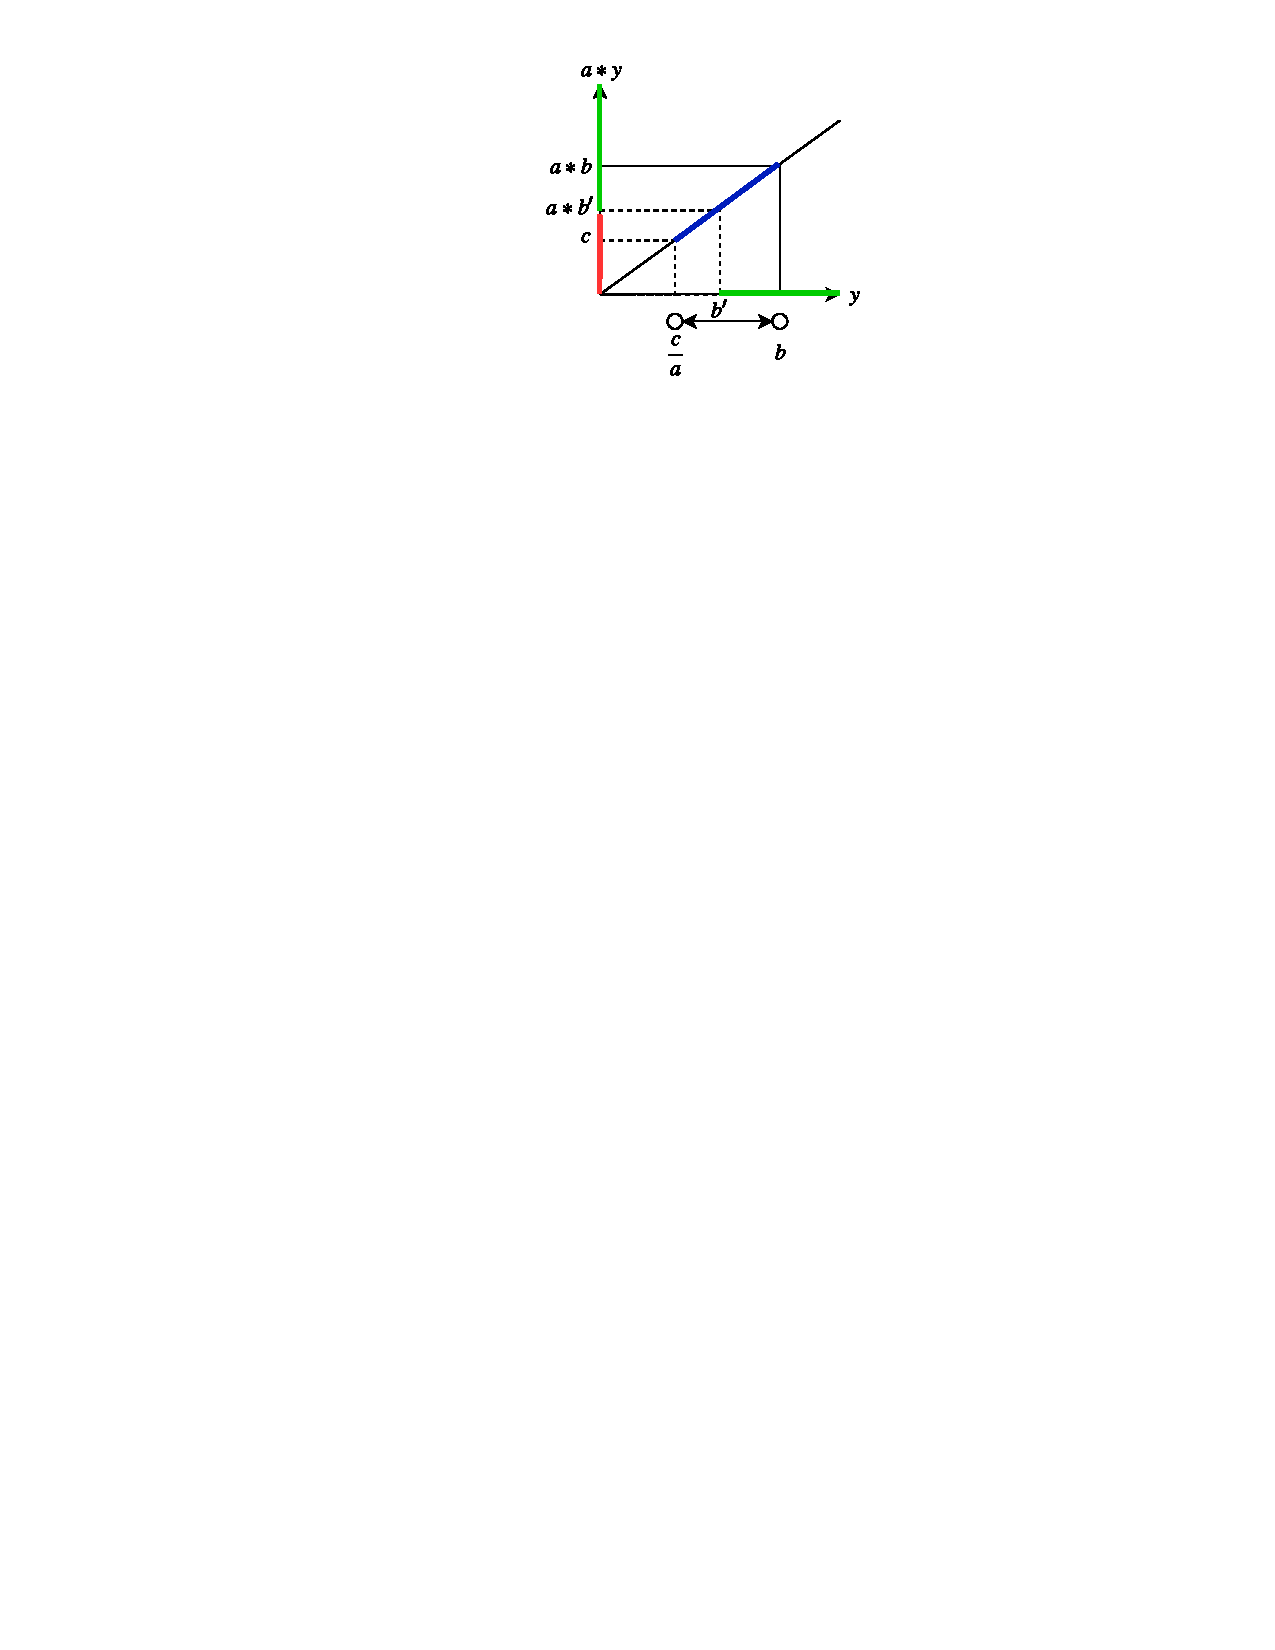
\includegraphics[width=0.6\linewidth]{./figures/ICP1_1.pdf}
  \caption{ICP 1.1}
  \label{fig:FixAModifyB}
\end{figure}

\begin{figure}[ht!]
  \centering
  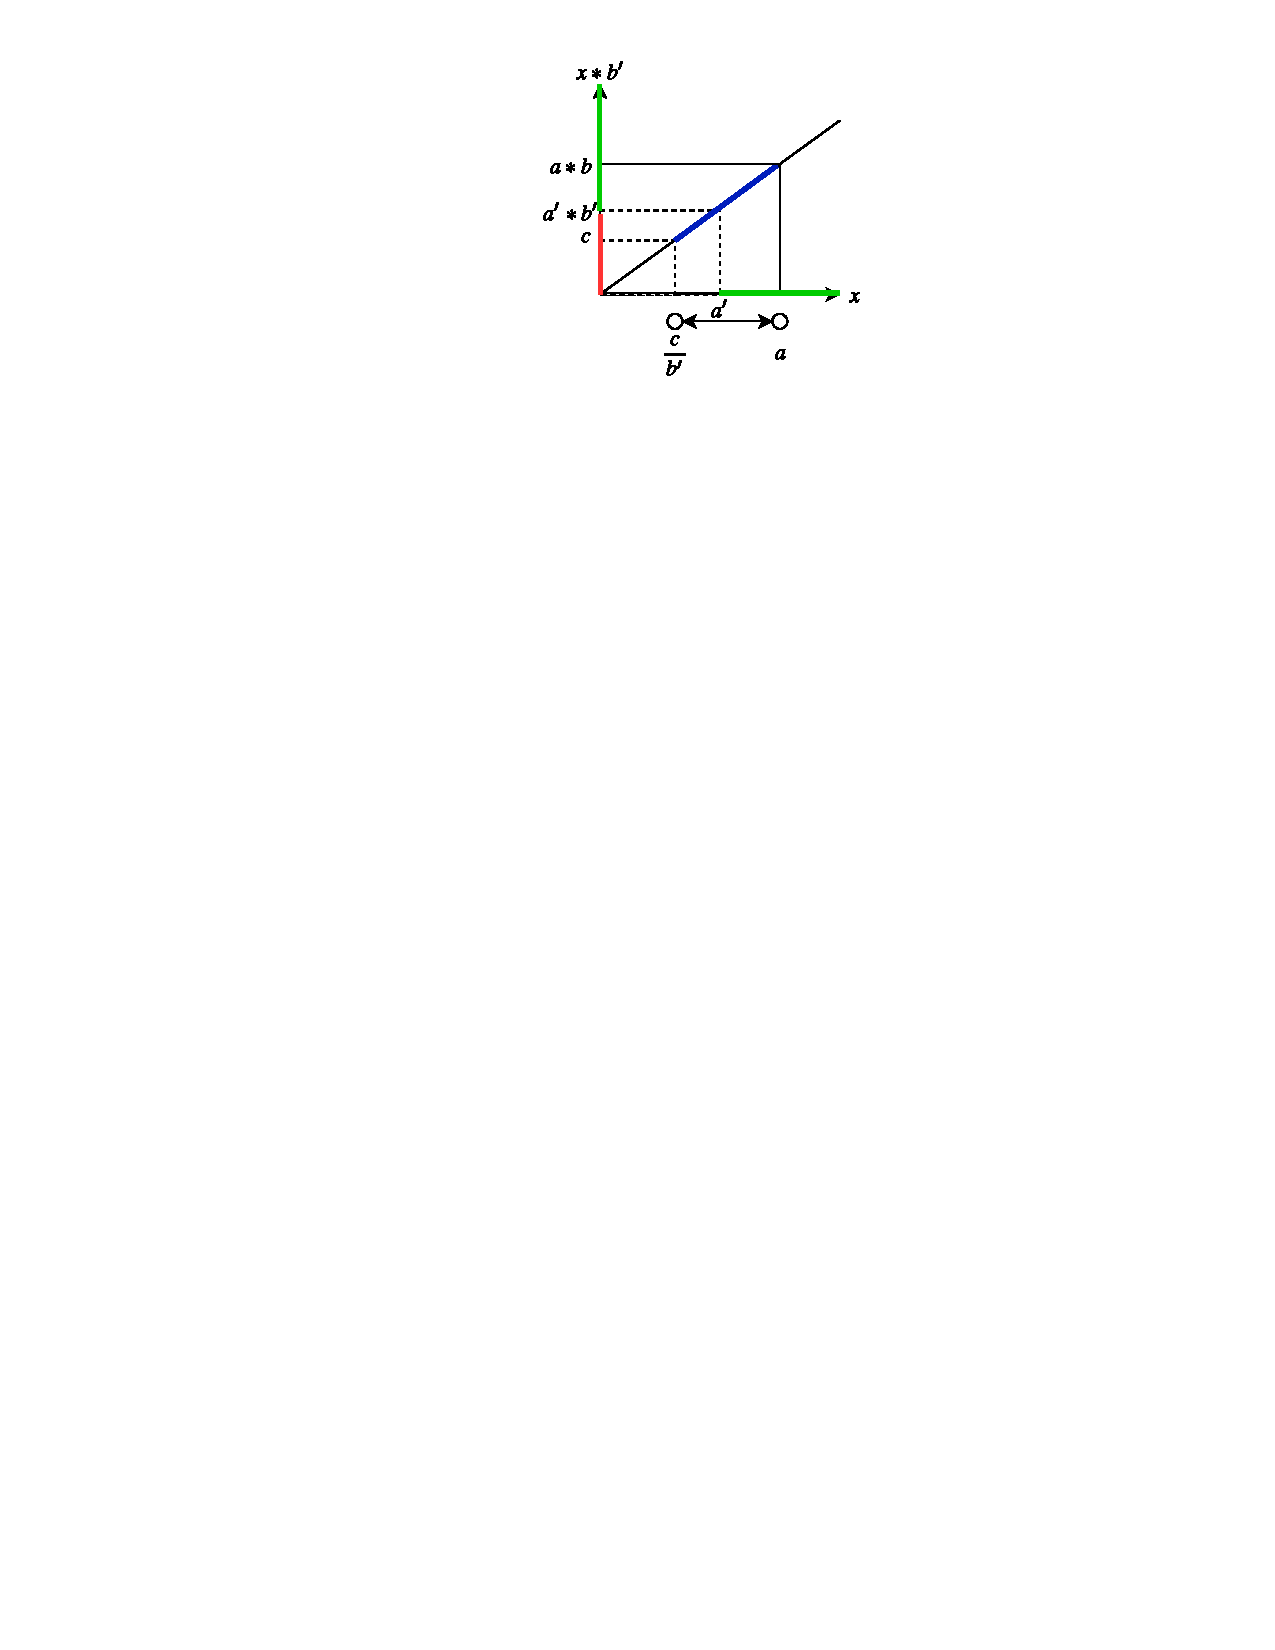
\includegraphics[width=0.6\linewidth]{./figures/ICP1_2.pdf}
  \caption{ICP 1.2}
  \label{fig:FixBModifyA}
\end{figure}

\noindent  Notice that $a$ and $b$ are positive and we know that their product is not $c$.\newline

\noindent  So, for $c < a \ast b$ we have two axioms, generalizing the above observations also to the negative domain (remember we defined $c^\prime = a^\prime \ast b^\prime$):

\begin{enumerate}
    \item $$((x \geq a^\prime \wedge y \geq b^\prime) \vee (x \leq -a^\prime \wedge y \leq -b^\prime)) \to (z \geq c^\prime)$$
    \item $$((x \geq a^\prime \wedge y \leq -b^\prime) \vee (x \leq -a^\prime \wedge y \geq b^\prime)) \to (z \leq -c^\prime)$$
\end{enumerate}

\noindent  Let us consider now $c > a \ast b$.
That means we guessed the product too high.
Dually to the previous case we take some values $a^\prime$ and $b^\prime$ above $a$ and $b$ respectively such that $a^\prime b^\prime$ is still below $c$ and state that for all pairs of values below $a^\prime$ and $b^\prime$ respectively, their product is less than $a^\prime b^\prime$.
This way, we say that $ab$ is at most $a^\prime b^\prime$.
So, $c$ will be excluded.\newline

\noindent In the same way, we can choose $a^\prime$ and $b^\prime$ either the minimum ($a$ and $b$, respectively) or arbitary near the maximum ($c + \epsilon$) or something in between:
\begin{itemize}
    \item $c > ab \text{ or, } b < \frac{c}{a}$ and $0 < b \leq b^\prime$\newline
    
    We choose, $b \leq b^\prime < \frac{c}{a}$
     \item $c > a^\prime b^\prime \text{ or, } a^\prime < \frac{c}{b^\prime}$ and $0 < a \leq a^\prime$\newline
     
     We choose, $a \leq a^\prime < \frac{c}{b^\prime}$
\end{itemize}

\noindent  So, for $c > ab$ we have one axiom, which covers also the case for zero values and the symmetric case for negative values:
$$(-a^\prime \leq x \leq a^\prime) \wedge (-b^\prime \leq y \leq b^\prime) \to (-c^\prime \leq z \leq c^\prime)$$

\noindent  $\textbf{Heuristics:}$ We have also contributed in this work by using different heuristics to identify the unsatisfied axioms.
Our main goal of using different heuristics in the refinement process is to identify unsatisfied axioms in a way so that the axiom generation is computationally not too expensive and adding them for refinement will exclude a relatively large or search-wise relevant" part of the state space.
In other words, different heuristics will help us to find the best way of refinement.
Generally, there is a maximum numbers of unsatisfied axioms we can use for refinement.
We may control the number of unsatisfied axioms to be added to $A$.
We can start checking with the easiest axiom. 
So, we check zero axiom for all formulas for all equalities.
If we find unsatisfied any zero axiom then we add it to the linearized formula and recheck.
We can also check any type of axioms regardless of whether the axiom is the easiest one for all equalities.
Then, collect all unsatisfied axioms to $A$ which are added to the linearized formula  and recheck.
Moreover, we can remove some unsatisfied axioms from $A$ before adding it to the linearized formula.
So, there is no specific rules to generate $A$.
If $A$ is not empty, we refine and continue. 
If $A$ is empty, we think about the next axiom type.\newline

\noindent We have tried different heuristics.
Then, we have tried to compare the running time so that we can decide what is better and which type of axioms to check first.
We have tried to come to a conclusion whether it is better to add always one unsatisfied axiom to $A$ or it is better to add one for each multiplication term or for some multiplication terms.
Basically, we play around because we know that we will not get the same solution for different heuristics.
It is completely up to us how we want to play with the axioms.
That is why, we try different ways to compute the running time and evaluate to find the best heuristic.\newline

\noindent So far, we have seen that we have generated five types of axioms in our work: zero axiom, monotonicity axiom, tangent plane axiom, congruence axiom and ICP axiom.
Each heuristic will be applied on different sequences of these axiom types for collecting unsatisfied axioms.
It is up to us how we want to make different sequences of axiom types.
We try to place the lightweighted axiom type first in the sequences.
We have used $7$ different sequences of axiom types:

\begin{enumerate}
    \item \textbf{Sequence $1$:} zero, tangent plane, ICP, congruence, monotonicity. \label{item:sequences}
    \item \textbf{Sequence $2$:} tangent plane, zero, ICP, congruence, monotonicity.
    \item \textbf{Sequence $3$:} tangent plane, ICP, zero, congruence, monotonicity.
    \item \textbf{Sequence $4$:} ICP, zero, tangent plane, congruence, monotonicity.
    \item \textbf{Sequence $5$:} ICP, tangent plane, zero, congruence, monotonicity.
    \item \textbf{Sequence $6$:} congruence, zero, tangent plane, ICP, monotonicity.
    \item \textbf{Sequence $7$:} monotonicity, zero, tangent plane, ICP, congruence.
\end{enumerate}

\noindent We decide to use $3$ different heuristics over each sequence of axiom types to perform the refinement process:

\begin{enumerate}
\label{item:heuristics}
    \item \textbf{Heuristic $1$:} Each loop will be run over the axioms following a given fixed order (one of the $7$ orders above).
    It will search in this order for an axiom instance that is violated by the solution for the abstraction.
    The first such axiom instance is added to $A$ and the refinement process terminates.
    \item \textbf{Heuristic $2$:} Similarly to $1$, but when a violating axiom instance is found then all violating instances of the given axiom are added to $A$.
    \item \textbf{Heuristic $3$:} Similarly to $2$ but here a percentage of unsatisfied axioms are deleted from $A$ randomly.
    We have also chosen this percentage randomly from $25\%$ to $50\%$ of the size of $A$.
\end{enumerate}

\noindent Notice that if we apply each heuristic over each sequence, we will get $21$ different solutions for $\hat{\varphi}$.
We compute running time and evalute it for different ways.
The evaluation result is discussed in the Chapter \ref{chap:experimental_result}.



